\documentclass[aspectratio=169, 10pt, t]{beamer}

% ==============================================================================
% PACKAGES & SYSTEM CONFIGURATION
% ==============================================================================
\usepackage[utf8]{inputenc}
\usepackage[T1]{fontenc}
\usepackage{lmodern}
\usepackage{graphicx}
\usepackage{tikz}
\usepackage{tcolorbox}
\usepackage{booktabs}
\usepackage{tabularx}
\usepackage{colortbl}
\usepackage{xcolor}
\usepackage{calc}
\usepackage{amsmath,amssymb}

\usetikzlibrary{calc, positioning, shapes.geometric, arrows.meta, backgrounds, fit}
\tcbuselibrary{skins, raster}

% ==============================================================================
% COLOR PALETTE (MINIMALIST CORPORATE SLATE & BLUE)
% ==============================================================================
\definecolor{primary}{HTML}{1E40AF}       % Corporate Deep Blue (Primary Accent)
\definecolor{darkslate}{HTML}{0F172A}     % Dark Slate (Headings & Primary Text)
\definecolor{mutedgray}{HTML}{475569}     % Slate 600 (Secondary & Body text)
\definecolor{lightgray}{HTML}{94A3B8}     % Slate 400 (Dividers & Sub-captions)
\definecolor{cardbg}{HTML}{F8FAFC}        % Slate 50 (Soft Neutral Card Background)
\definecolor{cardborder}{HTML}{E2E8F0}    % Slate 200 (Clean Hairline Border)
\definecolor{tableheader}{HTML}{F1F5F9}  % Slate 100 (Table Header Background)

% Subtle Functional Tints (Restrained, Never Over-Saturated)
\definecolor{problemtext}{HTML}{991B1B}   % Deep Maroon (Before / Issue Text)
\definecolor{problembg}{HTML}{FEF2F2}     % Soft Tint for Before Box
\definecolor{problemborder}{HTML}{FCA5A5} % Soft Border for Before Box

\definecolor{solutiontext}{HTML}{1E40AF}  % Deep Blue (After / Feature Text)
\definecolor{solutionbg}{HTML}{F8FAFC}    % Clean Slate for After Box
\definecolor{solutionborder}{HTML}{CBD5E1}% Clean Border for After Box

% Global Beamer Font Colors
\setbeamercolor{normal text}{fg=darkslate,bg=white}
\setbeamercolor{frametitle}{fg=darkslate,bg=white}
\setbeamercolor{footline}{fg=mutedgray,bg=white}
\setbeamercolor{background canvas}{bg=white}

% Disable Navigation Symbols
\setbeamertemplate{navigation symbols}{}

% Slide Geometry & Margins (16:9 Widescreen)
\setbeamersize{text margin left=0.7cm, text margin right=0.7cm}

% Custom Minimal Frametitle
\setbeamertemplate{frametitle}{%
    \vspace{0.35cm}%
    \begin{beamercolorbox}[wd=\paperwidth,leftskip=0.7cm,rightskip=0.7cm]{frametitle}%
        {\fontsize{13.5}{17}\selectfont\textbf{\insertframetitle}}\par%
        \ifx\insertframesubtitle\@empty\else%
            \vspace{2pt}%
            {\color{mutedgray}\fontsize{8.5}{11}\selectfont\insertframesubtitle}\par%
        \fi%
    \end{beamercolorbox}%
    \vspace{-0.15cm}%
}

% Custom Minimal Footline
\setbeamertemplate{footline}{%
    \ifnum\thepage>0%
    \begin{beamercolorbox}[wd=\paperwidth,ht=0.45cm,dp=0.2cm,leftskip=0.7cm,rightskip=0.7cm]{footline}%
        {\color{lightgray}\fontsize{7}{9}\selectfont\textbf{Spare Part EMS 2.0} \textbullet\ Improvement Report}%
        \hfill%
        {\color{lightgray}\fontsize{7}{9}\selectfont Slide \insertframenumber{} / \inserttotalframenumber}%
    \end{beamercolorbox}%
    \fi%
}

% ==============================================================================
% REUSABLE MINIMALIST BOX STYLES
% ==============================================================================

% Neutral Clean Card
\newtcolorbox{minimalcard}[1][]{
    colback=cardbg,
    colframe=cardborder,
    arc=3pt,
    boxrule=0.6pt,
    left=6pt, right=6pt, top=5pt, bottom=5pt,
    #1
}

% Restrained BEFORE Box
\newtcolorbox{beforebox}[1][]{
    colback=problembg,
    colframe=problemborder,
    coltitle=problemtext,
    fonttitle=\fontsize{7.5}{9.5}\bfseries\selectfont,
    title={\textbf{BEFORE}},
    arc=3pt,
    boxrule=0.6pt,
    left=6pt, right=6pt, top=4pt, bottom=4pt,
    #1
}

% Restrained AFTER Box
\newtcolorbox{afterbox}[1][]{
    colback=solutionbg,
    colframe=solutionborder,
    coltitle=primary,
    fonttitle=\fontsize{7.5}{9.5}\bfseries\selectfont,
    title={\textbf{AFTER}},
    arc=3pt,
    boxrule=0.6pt,
    left=6pt, right=6pt, top=4pt, bottom=4pt,
    #1
}

% ==============================================================================
% DOCUMENT BODY (COMBINED EXECUTIVE DECK: 8 SLIDES)
% ==============================================================================
\begin{document}

% ==============================================================================
% SLIDE 1 (COMBINED): TITLE, TODAY'S PROBLEM & 6 CONNECTED MODULES
% ==============================================================================
\begin{frame}[plain]
    \vspace{0.15cm}
    
    % Top Header Banner
    \begin{beamercolorbox}[wd=\textwidth]{plain}
        \tikz[baseline=-0.6ex]\node[fill=brandmint, text=brandnavy, rounded corners=2pt, inner xsep=5pt, inner ysep=2pt, font=\fontsize{7}{8.5}\bfseries\selectfont] {IMPROVEMENT REPORT};
        \hspace{4pt}
        {\fontsize{13}{16}\bfseries\selectfont\color{brandnavy}Spare Part EMS 2.0}
        \hspace{6pt}
        {\fontsize{8.5}{10.5}\selectfont\color{mutedgray}\textbar\hspace{6pt}One platform to manage the full spare part lifecycle}
    \end{beamercolorbox}
    
    \vspace{0.15cm}
    
    \begin{columns}[T]
        % ======================================================================
        % LEFT COLUMN: TODAY'S PAIN POINTS (OLD SLIDE 2)
        % ======================================================================
        \begin{column}{0.375\textwidth}
            % Section Header
            \tikz[baseline=-0.6ex]\node[fill=softred, text=brandorange, rounded corners=2pt, inner xsep=4pt, inner ysep=1.5pt, font=\fontsize{6.8}{8}\bfseries\selectfont] {TODAY'S PROCESS};
            \hspace{3pt}
            {\fontsize{8.5}{10.5}\bfseries\selectfont\color{slatenavy}Loses Data, Time \& Accuracy}\par
            \vspace{0.15cm}
            
            % 4 Slim Problem Cards
            \begin{tcolorbox}[
                colback=cardbg, colframe=cardborder, arc=3pt, boxrule=0.5pt,
                left=3.5pt, right=3.5pt, top=3pt, bottom=3pt, height=1.15cm
            ]
                \begin{columns}[c]
                    \begin{column}{0.18\textwidth}
                        \centering
                        
\includegraphics[height=0.58cm, keepaspectratio]{images/image-2-1.png}
                    \end{column}
                    \begin{column}{0.80\textwidth}
                        {\fontsize{7.5}{9}\bfseries\selectfont\color{slatenavy}Fragmented data}\par
                        {\fontsize{6.6}{8}\selectfont\color{mutedgray}Excel/legacy in parallel; 1 editor lock.}
                    \end{column}
                \end{columns}
            \end{tcolorbox}
            
            \vspace{0.06cm}
            
            \begin{tcolorbox}[
                colback=cardbg, colframe=cardborder, arc=3pt, boxrule=0.5pt,
                left=3.5pt, right=3.5pt, top=3pt, bottom=3pt, height=1.15cm
            ]
                \begin{columns}[c]
                    \begin{column}{0.18\textwidth}
                        \centering
                        
\includegraphics[height=0.58cm, keepaspectratio]{images/image-2-2.png}
                    \end{column}
                    \begin{column}{0.80\textwidth}
                        {\fontsize{7.5}{9}\bfseries\selectfont\color{slatenavy}Missed purchase info}\par
                        {\fontsize{6.6}{8}\selectfont\color{mutedgray}No bulk interlock/price check; high rejects.}
                    \end{column}
                \end{columns}
            \end{tcolorbox}
            
            \vspace{0.06cm}
            
            \begin{tcolorbox}[
                colback=cardbg, colframe=cardborder, arc=3pt, boxrule=0.5pt,
                left=3.5pt, right=3.5pt, top=3pt, bottom=3pt, height=1.15cm
            ]
                \begin{columns}[c]
                    \begin{column}{0.18\textwidth}
                        \centering
                        
\includegraphics[height=0.58cm, keepaspectratio]{images/image-2-3.png}
                    \end{column}
                    \begin{column}{0.80\textwidth}
                        {\fontsize{7.5}{9}\bfseries\selectfont\color{slatenavy}No cost control}\par
                        {\fontsize{6.6}{8}\selectfont\color{mutedgray}No live cost or over-budget view; manual ETA.}
                    \end{column}
                \end{columns}
            \end{tcolorbox}
            
            \vspace{0.06cm}
            
            \begin{tcolorbox}[
                colback=cardbg, colframe=cardborder, arc=3pt, boxrule=0.5pt,
                left=3.5pt, right=3.5pt, top=3pt, bottom=3pt, height=1.15cm
            ]
                \begin{columns}[c]
                    \begin{column}{0.18\textwidth}
                        \centering
                        
\includegraphics[height=0.58cm, keepaspectratio]{images/image-2-4.png}
                    \end{column}
                    \begin{column}{0.80\textwidth}
                        {\fontsize{7.5}{9}\bfseries\selectfont\color{slatenavy}Wrong EBOM and WO}\par
                        {\fontsize{6.6}{8}\selectfont\color{mutedgray}10 lines merged into 1 WO on wrong unit.}
                    \end{column}
                \end{columns}
            \end{tcolorbox}
        \end{column}
        
        \hspace{0.01\textwidth}
        
        % ======================================================================
        % RIGHT COLUMN: THE 6 CONNECTED MODULES (OLD SLIDE 3)
        % ======================================================================
        \begin{column}{0.605\textwidth}
            % Section Header
            \tikz[baseline=-0.6ex]\node[fill=softgreen, text=brandteal, rounded corners=2pt, inner xsep=4pt, inner ysep=1.5pt, font=\fontsize{6.8}{8}\bfseries\selectfont] {EMS 2.0 SOLUTION};
            \hspace{3pt}
            {\fontsize{8.5}{10.5}\bfseries\selectfont\color{slatenavy}One Platform, Six Connected Modules}\par
            \vspace{0.15cm}
            
            % Row 1: Modules 0, 1, 2
            \begin{columns}[T]
                % Module 0
                \begin{column}{0.318\textwidth}
                    \begin{tcolorbox}[
                        colback=cardbg, colframe=cardborder, arc=3pt, boxrule=0.5pt,
                        left=4pt, right=4pt, top=4pt, bottom=4pt, height=2.35cm
                    ]
                        \tikz[baseline=-0.5ex]\node[fill=brandteal, text=white, rounded corners=2pt, inner sep=1.8pt, font=\fontsize{6.8}{8}\bfseries\selectfont, minimum width=0.42cm, minimum height=0.42cm] {0};
                        \hspace{2pt}
                        {\fontsize{7.5}{9}\bfseries\selectfont\color{slatenavy}Forecast \& Stock}\par
                        \vspace{0.1cm}
                        {\fontsize{6.6}{8}\selectfont\color{mutedgray}
                        Predicts usage, triggers reorders and caps stock levels.
                        }
                    \end{tcolorbox}
                \end{column}
                
                % Module 1
                \begin{column}{0.318\textwidth}
                    \begin{tcolorbox}[
                        colback=cardbg, colframe=cardborder, arc=3pt, boxrule=0.5pt,
                        left=4pt, right=4pt, top=4pt, bottom=4pt, height=2.35cm
                    ]
                        \tikz[baseline=-0.5ex]\node[fill=brandteal, text=white, rounded corners=2pt, inner sep=1.8pt, font=\fontsize{6.8}{8}\bfseries\selectfont, minimum width=0.42cm, minimum height=0.42cm] {1};
                        \hspace{2pt}
                        {\fontsize{7.5}{9}\bfseries\selectfont\color{slatenavy}Mass Search}\par
                        \vspace{0.1cm}
                        {\fontsize{6.6}{8}\selectfont\color{mutedgray}
                        Price, interlock, photos and 4 PO routes in one view.
                        }
                    \end{tcolorbox}
                \end{column}
                
                % Module 2
                \begin{column}{0.318\textwidth}
                    \begin{tcolorbox}[
                        colback=cardbg, colframe=cardborder, arc=3pt, boxrule=0.5pt,
                        left=4pt, right=4pt, top=4pt, bottom=4pt, height=2.35cm
                    ]
                        \tikz[baseline=-0.5ex]\node[fill=brandteal, text=white, rounded corners=2pt, inner sep=1.8pt, font=\fontsize{6.8}{8}\bfseries\selectfont, minimum width=0.42cm, minimum height=0.42cm] {2};
                        \hspace{2pt}
                        {\fontsize{7.5}{9}\bfseries\selectfont\color{slatenavy}Purchasing Flow}\par
                        \vspace{0.1cm}
                        {\fontsize{6.6}{8}\selectfont\color{mutedgray}
                        Multi-user requests, auto-routing and an audit trail.
                        }
                    \end{tcolorbox}
                \end{column}
            \end{columns}
            
            \vspace{0.1cm}
            
            % Row 2: Modules 3, 4, 5
            \begin{columns}[T]
                % Module 3
                \begin{column}{0.318\textwidth}
                    \begin{tcolorbox}[
                        colback=cardbg, colframe=cardborder, arc=3pt, boxrule=0.5pt,
                        left=4pt, right=4pt, top=4pt, bottom=4pt, height=2.35cm
                    ]
                        \tikz[baseline=-0.5ex]\node[fill=brandteal, text=white, rounded corners=2pt, inner sep=1.8pt, font=\fontsize{6.8}{8}\bfseries\selectfont, minimum width=0.42cm, minimum height=0.42cm] {3};
                        \hspace{2pt}
                        {\fontsize{7.5}{9}\bfseries\selectfont\color{slatenavy}Cost \& ETA}\par
                        \vspace{0.1cm}
                        {\fontsize{6.6}{8}\selectfont\color{mutedgray}
                        ETA tracking, over-budget reasons, cost booked at issue.
                        }
                    \end{tcolorbox}
                \end{column}
                
                % Module 4
                \begin{column}{0.318\textwidth}
                    \begin{tcolorbox}[
                        colback=cardbg, colframe=cardborder, arc=3pt, boxrule=0.5pt,
                        left=4pt, right=4pt, top=4pt, bottom=4pt, height=2.35cm
                    ]
                        \tikz[baseline=-0.5ex]\node[fill=brandteal, text=white, rounded corners=2pt, inner sep=1.8pt, font=\fontsize{6.8}{8}\bfseries\selectfont, minimum width=0.42cm, minimum height=0.42cm] {4};
                        \hspace{2pt}
                        {\fontsize{7.5}{9}\bfseries\selectfont\color{slatenavy}EBOM}\par
                        \vspace{0.1cm}
                        {\fontsize{6.6}{8}\selectfont\color{mutedgray}
                        Visual line and mechanism tree with sanity rules.
                        }
                    \end{tcolorbox}
                \end{column}
                
                % Module 5
                \begin{column}{0.318\textwidth}
                    \begin{tcolorbox}[
                        colback=cardbg, colframe=cardborder, arc=3pt, boxrule=0.5pt,
                        left=4pt, right=4pt, top=4pt, bottom=4pt, height=2.35cm
                    ]
                        \tikz[baseline=-0.5ex]\node[fill=brandteal, text=white, rounded corners=2pt, inner sep=1.8pt, font=\fontsize{6.8}{8}\bfseries\selectfont, minimum width=0.42cm, minimum height=0.42cm] {5};
                        \hspace{2pt}
                        {\fontsize{7.5}{9}\bfseries\selectfont\color{slatenavy}Work Orders}\par
                        \vspace{0.1cm}
                        {\fontsize{6.6}{8}\selectfont\color{mutedgray}
                        Mass WO creation with correct mechanism allocation.
                        }
                    \end{tcolorbox}
                \end{column}
            \end{columns}
        \end{column}
    \end{columns}
\end{frame}

% ==============================================================================
% SLIDE 4: BEFORE AND AFTER AT A GLANCE (COMPARISON TABLE)
% ==============================================================================
\begin{frame}{Before and after at a glance}
    \vspace{0.1cm}
    
    \renewcommand{\arraystretch}{1.22}
    {\fontsize{7.5}{9.5}\selectfont
    \begin{tabularx}{\textwidth}{
        >{\bfseries\color{slatenavy}}p{1.9cm}
        >{\color{mutedgray}}X
        >{\color{slatenavy}}X
        >{\bfseries\color{brandteal}}p{3.2cm}
    }
        \toprule
        \rowcolor{tableheader}
        \textcolor{slatenavy}{\textbf{Area}} & 
        \textcolor{brandorange}{\textbf{Before}} & 
        \textcolor{brandteal}{\textbf{After}} & 
        \textcolor{slatenavy}{\textbf{Impact}} \\
        \midrule
        
        0 \hspace{3pt} Planning &
        Reactive; no forecast or safety stock &
        Auto forecast, reorder alerts, stock cap &
        \tikz[baseline=-0.5ex]\node[fill=softgreen, text=brandteal, rounded corners=2pt, inner xsep=4pt, inner ysep=1.5pt] {Proactive planning}; \\
        
        1 \hspace{3pt} Search &
        Excel plus legacy system; no bulk lookup &
        Bulk lookup of price, interlock, photos, 4 PO routes &
        \tikz[baseline=-0.5ex]\node[fill=softgreen, text=brandteal, rounded corners=2pt, inner xsep=4pt, inner ysep=1.5pt] {$-$80\% lookup time}; \\
        
        2 \hspace{3pt} Purchasing &
        One editor per file; rejects get missed &
        Real-time multi-user; bulk handling; audit log &
        \tikz[baseline=-0.5ex]\node[fill=softgreen, text=brandteal, rounded corners=2pt, inner xsep=4pt, inner ysep=1.5pt] {No file locks, no lost orders}; \\
        
        3 \hspace{3pt} ETA \& cost &
        ETA via intermediaries; no live cost view &
        Direct ETA updates; overdue alerts; cost at issue &
        \tikz[baseline=-0.5ex]\node[fill=softgreen, text=brandteal, rounded corners=2pt, inner xsep=4pt, inner ysep=1.5pt] {Real-time budget control}; \\
        
        4 \hspace{3pt} EBOM &
        Hard to read; missing groups unnoticed &
        Visual tree; sanity rules; fast cloning &
        \tikz[baseline=-0.5ex]\node[fill=softgreen, text=brandteal, rounded corners=2pt, inner xsep=4pt, inner ysep=1.5pt] {Standardized EBOM data}; \\
        
        5 \hspace{3pt} Work Orders &
        Manual; 1 WO covers 10 lines &
        Bulk WO split by line and mechanism &
        \tikz[baseline=-0.5ex]\node[fill=softgreen, text=brandteal, rounded corners=2pt, inner xsep=4pt, inner ysep=1.5pt] {Accurate MTBF / MTTR}; \\
        
        \bottomrule
    \end{tabularx}
    }
\end{frame}

% ==============================================================================
% SLIDE 3: MODULES 0-1 (PLAN AHEAD, CHECK BEFORE ORDERING)
% ==============================================================================
\begin{frame}{Modules 0–1: Plan ahead, check before ordering}
    \vspace{0.15cm}
    
    \begin{columns}[T]
        % Module 0: Forecast & Safety Stock
        \begin{column}{0.485\textwidth}
            {\fontsize{9.5}{12}\bfseries\selectfont\color{primary}0 \textbullet\ Forecast \& Safety Stock}\par
            \vspace{0.2cm}
            
            % BEFORE Box
            \begin{beforebox}
                {\fontsize{7.8}{10.5}\selectfont\color{darkslate}
                \begin{itemize}\setlength{\itemsep}{2pt}\setlength{\leftmargin}{10pt}
                    \item[\textcolor{problemtext}{\textbullet}] No usage forecast; ordering is reactive
                    \item[\textcolor{problemtext}{\textbullet}] Long-lead parts are ordered too late
                    \item[\textcolor{problemtext}{\textbullet}] No safety stock: over- or under-buying
                \end{itemize}
                }
            \end{beforebox}
            
            \vspace{0.15cm}
            
            % AFTER Box
            \begin{afterbox}
                {\fontsize{7.8}{10.5}\selectfont\color{darkslate}
                \begin{itemize}\setlength{\itemsep}{2pt}\setlength{\leftmargin}{10pt}
                    \item[\textcolor{primary}{\textbullet}] Auto forecast from production output and time
                    \item[\textcolor{primary}{\textbullet}] Automated reorder alerts when an order is due
                    \item[\textcolor{primary}{\textbullet}] Safety-stock limit configured per part
                    \item[\textcolor{primary}{\textbullet}] Bulk Q-Code onboarding and registration
                \end{itemize}
                }
            \end{afterbox}
        \end{column}
        
        % Module 1: Mass Search
        \begin{column}{0.485\textwidth}
            {\fontsize{9.5}{12}\bfseries\selectfont\color{primary}1 \textbullet\ Mass Search}\par
            \vspace{0.2cm}
            
            % BEFORE Box
            \begin{beforebox}
                {\fontsize{7.8}{10.5}\selectfont\color{darkslate}
                \begin{itemize}\setlength{\itemsep}{2pt}\setlength{\leftmargin}{10pt}
                    \item[\textcolor{problemtext}{\textbullet}] Excel and legacy system checked separately
                    \item[\textcolor{problemtext}{\textbullet}] One item at a time; no bulk lookup capability
                    \item[\textcolor{problemtext}{\textbullet}] Orders rejected downstream after registration
                \end{itemize}
                }
            \end{beforebox}
            
            \vspace{0.15cm}
            
            % AFTER Box
            \begin{afterbox}
                {\fontsize{7.8}{10.5}\selectfont\color{darkslate}
                \begin{itemize}\setlength{\itemsep}{2pt}\setlength{\leftmargin}{10pt}
                    \item[\textcolor{primary}{\textbullet}] Bulk lookup: price, interlock, stock, photos
                    \item[\textcolor{primary}{\textbullet}] Status of all 4 PO routes visible in one view
                    \item[\textcolor{primary}{\textbullet}] Critical part issues flagged before ordering
                \end{itemize}
                }
            \end{afterbox}
        \end{column}
    \end{columns}
\end{frame}

% ==============================================================================
% SLIDE 4: MODULE 2 (FOUR PO ROUTES, AUTO-ESCALATED)
% ==============================================================================
\begin{frame}{Module 2: Four PO routes, auto-escalated}
    \vspace{0.1cm}
    
    % Top Waterfall Steps (4 Escalation Steps)
    \centering
    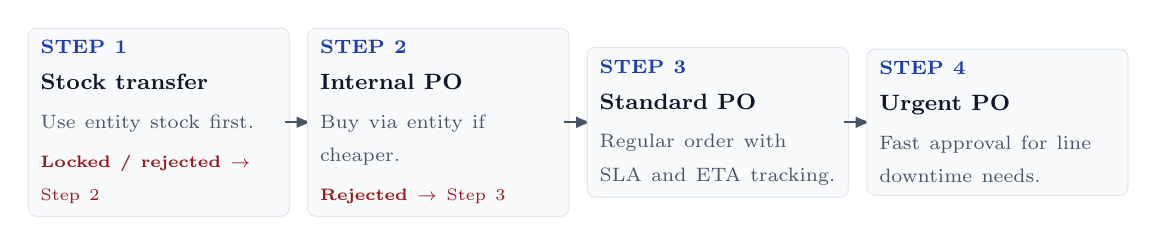
\begin{tikzpicture}[x=1cm, y=1cm]
        % Step 1: Stock Transfer
        \node[
            fill=cardbg, draw=cardborder, rounded corners=3pt,
            text width=3.0cm, inner sep=4.5pt, minimum height=1.65cm, align=left
        ] (s1) at (0, 0) {
            {\fontsize{7}{8.5}\bfseries\selectfont\color{primary}STEP 1}\par
            \vspace{1pt}
            {\fontsize{8.5}{10.5}\bfseries\selectfont\color{darkslate}Stock transfer}\par
            \vspace{2pt}
            {\fontsize{7}{8.5}\selectfont\color{mutedgray}Use entity stock first.}\par
            \vspace{2pt}
            {\fontsize{6.5}{8}\selectfont\color{problemtext}\textbf{Locked / rejected} $\rightarrow$ Step 2}
        };
        
        % Arrow 1 -> 2
        \draw[-{Latex[length=2mm]}, mutedgray, line width=0.7pt] (1.6, 0) -- (1.95, 0);
        
        % Step 2: Internal PO
        \node[
            fill=cardbg, draw=cardborder, rounded corners=3pt,
            text width=3.0cm, inner sep=4.5pt, minimum height=1.65cm, align=left
        ] (s2) at (3.55, 0) {
            {\fontsize{7}{8.5}\bfseries\selectfont\color{primary}STEP 2}\par
            \vspace{1pt}
            {\fontsize{8.5}{10.5}\bfseries\selectfont\color{darkslate}Internal PO}\par
            \vspace{2pt}
            {\fontsize{7}{8.5}\selectfont\color{mutedgray}Buy via entity if cheaper.}\par
            \vspace{2pt}
            {\fontsize{6.5}{8}\selectfont\color{problemtext}\textbf{Rejected} $\rightarrow$ Step 3}
        };
        
        % Arrow 2 -> 3
        \draw[-{Latex[length=2mm]}, mutedgray, line width=0.7pt] (5.15, 0) -- (5.5, 0);
        
        % Step 3: Standard PO
        \node[
            fill=cardbg, draw=cardborder, rounded corners=3pt,
            text width=3.0cm, inner sep=4.5pt, minimum height=1.65cm, align=left
        ] (s3) at (7.1, 0) {
            {\fontsize{7}{8.5}\bfseries\selectfont\color{primary}STEP 3}\par
            \vspace{1pt}
            {\fontsize{8.5}{10.5}\bfseries\selectfont\color{darkslate}Standard PO}\par
            \vspace{2pt}
            {\fontsize{7}{8.5}\selectfont\color{mutedgray}Regular order with SLA and ETA tracking.}
        };
        
        % Arrow 3 -> 4
        \draw[-{Latex[length=2mm]}, mutedgray, line width=0.7pt] (8.7, 0) -- (9.05, 0);
        
        % Step 4: Urgent PO
        \node[
            fill=cardbg, draw=cardborder, rounded corners=3pt,
            text width=3.0cm, inner sep=4.5pt, minimum height=1.65cm, align=left
        ] (s4) at (10.65, 0) {
            {\fontsize{7}{8.5}\bfseries\selectfont\color{primary}STEP 4}\par
            \vspace{1pt}
            {\fontsize{8.5}{10.5}\bfseries\selectfont\color{darkslate}Urgent PO}\par
            \vspace{2pt}
            {\fontsize{7}{8.5}\selectfont\color{mutedgray}Fast approval for line downtime needs.}
        };
    \end{tikzpicture}
    
    \vspace{0.25cm}
    
    % Bottom Comparison
    \begin{columns}[T]
        % BEFORE Box
        \begin{column}{0.485\textwidth}
            \begin{beforebox}
                {\fontsize{7.5}{10}\selectfont\color{darkslate}
                \begin{itemize}\setlength{\itemsep}{2pt}\setlength{\leftmargin}{10pt}
                    \item[\textcolor{problemtext}{\textbullet}] One Excel editor at a time (U-dock file lock)
                    \item[\textcolor{problemtext}{\textbullet}] Multi-layer review: LEC, Reviewer, Requestor
                    \item[\textcolor{problemtext}{\textbullet}] Rejects rechecked by hand; information gets lost
                    \item[\textcolor{problemtext}{\textbullet}] ETA chased manually through intermediaries
                \end{itemize}
                }
            \end{beforebox}
        \end{column}
        
        % AFTER Box
        \begin{column}{0.485\textwidth}
            \begin{afterbox}
                {\fontsize{7.5}{10}\selectfont\color{darkslate}
                \begin{itemize}\setlength{\itemsep}{2pt}\setlength{\leftmargin}{10pt}
                    \item[\textcolor{primary}{\textbullet}] Real-time multi-user work; replaces U-dock
                    \item[\textcolor{primary}{\textbullet}] LEC handles hundreds of items in bulk
                    \item[\textcolor{primary}{\textbullet}] In-system comments with an immutable audit trail
                    \item[\textcolor{primary}{\textbullet}] Overdue orders highlighted; ETA updated in-system
                \end{itemize}
                }
            \end{afterbox}
        \end{column}
    \end{columns}
\end{frame}

% ==============================================================================
% SLIDE 7: MODULE 3 (COST COUNTED WHEN PARTS ARE USED)
% ==============================================================================
\begin{frame}{Module 3: Cost counted when parts are used}
    \vspace{0.15cm}
    
    \begin{columns}[T]
        % Left Column: TODAY (Pain Points)
        \begin{column}{0.36\textwidth}
            \begin{tcolorbox}[
                colback=softred,
                colframe=brandorange!70,
                coltitle=brandorange,
                fonttitle=\fontsize{9}{11}\bfseries\selectfont,
                title={\textbf{TODAY}},
                arc=4pt,
                boxrule=0.8pt,
                left=8pt, right=8pt, top=8pt, bottom=8pt,
                height=5.1cm
            ]
                {\fontsize{8}{11}\selectfont
                \begin{itemize}\setlength{\itemsep}{5pt}\setlength{\leftmargin}{12pt}
                    \item[\textcolor{brandorange}{\textbullet}] No real-time cost or over-budget tracking
                    \item[\textcolor{brandorange}{\textbullet}] Cost not tied to the actual physical issue date
                    \item[\textcolor{brandorange}{\textbullet}] Orders disconnected from stock and budget
                    \item[\textcolor{brandorange}{\textbullet}] No view of issue-plan status per item
                \end{itemize}
                }
            \end{tcolorbox}
        \end{column}
        
        % Right Column: 4 Solution Pillars (2x2 Grid)
        \begin{column}{0.61\textwidth}
            % Row 1
            \begin{columns}[T]
                \begin{column}{0.485\textwidth}
                    \begin{tcolorbox}[
                        colback=cardbg, colframe=cardborder, arc=4pt, boxrule=0.7pt,
                        left=7pt, right=7pt, top=6pt, bottom=6pt, height=2.45cm
                    ]
                        \tikz[baseline=-0.5ex]\node[fill=brandteal, text=white, rounded corners=2pt, inner sep=2pt, font=\fontsize{7.5}{9}\bfseries\selectfont] {1};
                        \hspace{3pt}
                        {\fontsize{8.5}{10.5}\bfseries\selectfont\color{slatenavy}Cost on consumption}\par
                        \vspace{0.15cm}
                        {\fontsize{7.5}{9.5}\selectfont\color{mutedgray}
                        Cost is booked only when a part is issued, so each period's budget is accurate.
                        }
                    \end{tcolorbox}
                \end{column}
                
                \begin{column}{0.485\textwidth}
                    \begin{tcolorbox}[
                        colback=cardbg, colframe=cardborder, arc=4pt, boxrule=0.7pt,
                        left=7pt, right=7pt, top=6pt, bottom=6pt, height=2.45cm
                    ]
                        \tikz[baseline=-0.5ex]\node[fill=brandteal, text=white, rounded corners=2pt, inner sep=2pt, font=\fontsize{7.5}{9}\bfseries\selectfont] {2};
                        \hspace{3pt}
                        {\fontsize{8.5}{10.5}\bfseries\selectfont\color{slatenavy}ETA \& scheduling}\par
                        \vspace{0.15cm}
                        {\fontsize{7.5}{9.5}\selectfont\color{mutedgray}
                        Track arrival dates and schedule orders without cost spikes.
                        }
                    \end{tcolorbox}
                \end{column}
            \end{columns}
            
            \vspace{0.2cm}
            
            % Row 2
            \begin{columns}[T]
                \begin{column}{0.485\textwidth}
                    \begin{tcolorbox}[
                        colback=cardbg, colframe=cardborder, arc=4pt, boxrule=0.7pt,
                        left=7pt, right=7pt, top=6pt, bottom=6pt, height=2.45cm
                    ]
                        \tikz[baseline=-0.5ex]\node[fill=brandteal, text=white, rounded corners=2pt, inner sep=2pt, font=\fontsize{7.5}{9}\bfseries\selectfont] {3};
                        \hspace{3pt}
                        {\fontsize{8.5}{10.5}\bfseries\selectfont\color{slatenavy}Over-budget control}\par
                        \vspace{0.15cm}
                        {\fontsize{7.5}{9.5}\selectfont\color{mutedgray}
                        Live budget view. A mandatory reason code is required for every overrun.
                        }
                    \end{tcolorbox}
                \end{column}
                
                \begin{column}{0.485\textwidth}
                    \begin{tcolorbox}[
                        colback=cardbg, colframe=cardborder, arc=4pt, boxrule=0.7pt,
                        left=7pt, right=7pt, top=6pt, bottom=6pt, height=2.45cm
                    ]
                        \tikz[baseline=-0.5ex]\node[fill=brandteal, text=white, rounded corners=2pt, inner sep=2pt, font=\fontsize{7.5}{9}\bfseries\selectfont] {4};
                        \hspace{3pt}
                        {\fontsize{8.5}{10.5}\bfseries\selectfont\color{slatenavy}Issue-plan tracking}\par
                        \vspace{0.15cm}
                        {\fontsize{7.5}{9.5}\selectfont\color{mutedgray}
                        Every item shows clearly as planned, issued, or not issued.
                        }
                    \end{tcolorbox}
                \end{column}
            \end{columns}
        \end{column}
    \end{columns}
\end{frame}


% ==============================================================================
% SLIDE 6: MODULE 4 (EBOM YOU CAN SEE AND TRUST)
% ==============================================================================
\begin{frame}{Module 4: EBOM you can see and trust}
    \vspace{0.1cm}
    
    \begin{columns}[T]
        % Left Column: Visual EBOM Tree & Sanity Check
        \begin{column}{0.485\textwidth}
            \begin{tcolorbox}[
                colback=cardbg, colframe=cardborder, arc=4pt, boxrule=0.6pt,
                left=8pt, right=8pt, top=7pt, bottom=7pt, height=5.0cm
            ]
                % Production Lines
                {\fontsize{7}{8.5}\bfseries\selectfont\color{lightgray}PRODUCTION LINES}\par
                \vspace{2pt}
                \tikz[baseline=-0.5ex]{
                    \node[fill=white, draw=cardborder, text=primary, rounded corners=2pt, font=\fontsize{7}{8.5}\bfseries\selectfont, inner sep=3pt] {Line A};
                    \node[fill=white, draw=cardborder, text=mutedgray, rounded corners=2pt, font=\fontsize{7}{8.5}\selectfont, inner sep=3pt, right=4pt] at (1.1,0) {Line B};
                    \node[fill=white, draw=cardborder, text=mutedgray, rounded corners=2pt, font=\fontsize{7}{8.5}\selectfont, inner sep=3pt, right=4pt] at (2.2,0) {Line C};
                }
                
                \vspace{0.2cm}
                
                % Mechanism
                {\fontsize{7}{8.5}\bfseries\selectfont\color{lightgray}MECHANISM}\par
                \vspace{2pt}
                {\fontsize{8.5}{10.5}\bfseries\selectfont\color{darkslate}Mechanism / Sub-assembly}\par
                
                \vspace{0.25cm}
                
                % 3 Component Group Checks (Sensor, Cable, Actuator)
                \begin{columns}[T]
                    % Sensor
                    \begin{column}{0.31\textwidth}
                        \centering
                        
\includegraphics[height=0.75cm, keepaspectratio]{images/image-8-1.png}\par
                        \vspace{2pt}
                        {\fontsize{7.2}{8.5}\bfseries\selectfont Sensor}\par
                        \vspace{1pt}
                        {\fontsize{6.5}{8}\selectfont\color{mutedgray}Registered}
                    \end{column}
                    
                    % Cable
                    \begin{column}{0.31\textwidth}
                        \centering
                        
\includegraphics[height=0.75cm, keepaspectratio]{images/image-8-2.png}\par
                        \vspace{2pt}
                        {\fontsize{7.2}{8.5}\bfseries\selectfont Cable}\par
                        \vspace{1pt}
                        {\fontsize{6.5}{8}\selectfont\color{mutedgray}Registered}
                    \end{column}
                    
                    % Actuator
                    \begin{column}{0.31\textwidth}
                        \centering
                        
\includegraphics[height=0.75cm, keepaspectratio]{images/image-8-3.png}\par
                        \vspace{2pt}
                        {\fontsize{7.2}{8.5}\bfseries\selectfont Actuator}\par
                        \vspace{1pt}
                        {\fontsize{6.5}{8}\bfseries\selectfont\color{problemtext}Missing!}
                    \end{column}
                \end{columns}
                
                \vspace{0.35cm}
                % Sanity Check Progress Bar
                \tikz[x=1cm, y=1cm]{
                    \fill[white, rounded corners=2pt] (0,0) rectangle (5.8, 0.22);
                    \fill[primary, rounded corners=2pt] (0,0) rectangle (3.86, 0.22);
                    \node[anchor=west, font=\fontsize{6.8}{8}\bfseries\selectfont, text=darkslate] at (0, 0.42) {Completion: 2 of 3 required groups (67\%)};
                }
            \end{tcolorbox}
        \end{column}
        
        % Right Column: TODAY vs WHAT CHANGES
        \begin{column}{0.485\textwidth}
            % TODAY Box
            \begin{beforebox}[title={\textbf{TODAY}}]
                {\fontsize{7.5}{10}\selectfont\color{darkslate}
                \begin{itemize}\setlength{\itemsep}{2pt}\setlength{\leftmargin}{10pt}
                    \item[\textcolor{problemtext}{\textbullet}] No overview across parallel lines and mechanisms
                    \item[\textcolor{problemtext}{\textbullet}] Wrong or missing part groups go completely unnoticed
                    \item[\textcolor{problemtext}{\textbullet}] No bulk registration or visual progress tracking
                \end{itemize}
                }
            \end{beforebox}
            
            \vspace{0.15cm}
            
            % WHAT CHANGES Box
            \begin{afterbox}[title={\textbf{WHAT CHANGES}}]
                {\fontsize{7.5}{10}\selectfont\color{darkslate}
                \begin{itemize}\setlength{\itemsep}{2pt}\setlength{\leftmargin}{10pt}
                    \item[\textcolor{primary}{\textbullet}] Visual view of all lines and mechanism trees
                    \item[\textcolor{primary}{\textbullet}] Sanity rules flag missing groups (Sensor, Cable, Actuator)
                    \item[\textcolor{primary}{\textbullet}] Mass cloning across identical lines in a single step
                    \item[\textcolor{primary}{\textbullet}] Real-time completion \% per mechanism and line
                \end{itemize}
                }
            \end{afterbox}
        \end{column}
    \end{columns}
\end{frame}

% ==============================================================================
% SLIDE 9: MODULE 5 (ONE ACTION, EVERY WORK ORDER)
% ==============================================================================
\begin{frame}{Module 5: One action, every work order}
    \vspace{0.05cm}
    
    % Top Section: Visual Comparison (10 lines WO allocation)
    \begin{columns}[T]
        % BEFORE
        \begin{column}{0.485\textwidth}
            \begin{tcolorbox}[
                colback=softred, colframe=brandorange!70, arc=4pt, boxrule=0.8pt,
                left=7pt, right=7pt, top=5pt, bottom=5pt, height=2.4cm
            ]
                {\fontsize{7.5}{9}\bfseries\selectfont\color{brandorange}BEFORE}\par
                \vspace{2pt}
                {\fontsize{8}{10}\selectfont\color{mutedgray}10 lines use the part}\par
                \vspace{3pt}
                \tikz[baseline=-0.5ex]\node[fill=brandorange!20, text=brandorange, rounded corners=2pt, font=\fontsize{8}{10}\bfseries\selectfont, inner sep=3pt] {1 WO $\longrightarrow$ 1 mechanism};
                \par
                \vspace{3pt}
                {\fontsize{7.5}{9.5}\bfseries\selectfont\color{brandorange}Line 1 shows 10$\times$ the cost; the other 9 show zero}
            \end{tcolorbox}
        \end{column}
        
        % AFTER
        \begin{column}{0.485\textwidth}
            \begin{tcolorbox}[
                colback=softgreen, colframe=brandteal!70, arc=4pt, boxrule=0.8pt,
                left=7pt, right=7pt, top=5pt, bottom=5pt, height=2.4cm
            ]
                {\fontsize{7.5}{9}\bfseries\selectfont\color{brandteal}AFTER}\par
                \vspace{2pt}
                {\fontsize{8}{10}\selectfont\color{mutedgray}10 lines use the part}\par
                \vspace{3pt}
                \tikz[baseline=-0.5ex]\node[fill=brandteal!20, text=brandteal, rounded corners=2pt, font=\fontsize{8}{10}\bfseries\selectfont, inner sep=3pt] {10 WOs, each on its own mechanism};
                \par
                \vspace{3pt}
                {\fontsize{7.5}{9.5}\bfseries\selectfont\color{brandteal}100\% precise cost allocation per line \& mechanism}
            \end{tcolorbox}
        \end{column}
    \end{columns}
    
    \vspace{0.25cm}
    
    % Bottom Section: 3 Feature Cards
    \begin{columns}[T]
        % Card 1
        \begin{column}{0.315\textwidth}
            \begin{tcolorbox}[
                colback=cardbg, colframe=cardborder, arc=4pt, boxrule=0.7pt,
                left=7pt, right=7pt, top=7pt, bottom=7pt, height=2.3cm
            ]
                {\fontsize{9}{11}\bfseries\selectfont\color{slatenavy}Less manual work}\par
                \vspace{0.2cm}
                {\fontsize{8}{10.5}\selectfont\color{mutedgray}
                One single action automatically generates and releases all work orders simultaneously.
                }
            \end{tcolorbox}
        \end{column}
        
        % Card 2
        \begin{column}{0.315\textwidth}
            \begin{tcolorbox}[
                colback=cardbg, colframe=cardborder, arc=4pt, boxrule=0.7pt,
                left=7pt, right=7pt, top=7pt, bottom=7pt, height=2.3cm
            ]
                {\fontsize{9}{11}\bfseries\selectfont\color{slatenavy}Correct allocation}\par
                \vspace{0.2cm}
                {\fontsize{8}{10.5}\selectfont\color{mutedgray}
                Parts post accurately to the specific mechanism of the exact line that consumed them.
                }
            \end{tcolorbox}
        \end{column}
        
        % Card 3
        \begin{column}{0.315\textwidth}
            \begin{tcolorbox}[
                colback=cardbg, colframe=cardborder, arc=4pt, boxrule=0.7pt,
                left=7pt, right=7pt, top=7pt, bottom=7pt, height=2.3cm
            ]
                {\fontsize{9}{11}\bfseries\selectfont\color{slatenavy}Reliable history}\par
                \vspace{0.2cm}
                {\fontsize{8}{10.5}\selectfont\color{mutedgray}
                Issuance data matches shop floor reality for exact MTBF/MTTR and audit compliance.
                }
            \end{tcolorbox}
        \end{column}
    \end{columns}
\end{frame}


% ==============================================================================
% SLIDE 10: EXECUTIVE IMPACT SUMMARY
% ==============================================================================
{
\setbeamercolor{background canvas}{bg=brandnavy}
\begin{frame}[plain]
    \vspace{0.7cm}
    
    % Category Badge
    \tikz\node[fill=brandmint, text=brandnavy, rounded corners=3pt, inner xsep=8pt, inner ysep=3pt, font=\fontsize{8}{10}\bfseries\selectfont] {BUSINESS VALUE};
    
    \vspace{0.3cm}
    
    {\fontsize{22}{26}\bfseries\selectfont\color{white}Impact: faster, more accurate, fully traceable}\par
    
    \vspace{0.6cm}
    
    % 4 Pillars of Value
    \begin{columns}[T]
        % Pillar 1: SPEED
        \begin{column}{0.235\textwidth}
            \begin{tcolorbox}[
                colback=white!10, colframe=white!20, arc=4pt, boxrule=0.7pt,
                left=7pt, right=7pt, top=7pt, bottom=7pt, height=4.2cm
            ]
                {\fontsize{7.5}{9}\bfseries\selectfont\color{brandmint}01 \textbullet\ SPEED}\par
                \vspace{4pt}
                {\fontsize{9}{11}\bfseries\selectfont\color{white}No more Excel file locks}\par
                \vspace{6pt}
                {\fontsize{7.8}{10}\selectfont\color{white!80}
                Mass Search, Request, EBOM and WO cut manual operations by \textbf{\color{brandmint}60--70\%}.
                }
            \end{tcolorbox}
        \end{column}
        
        % Pillar 2: ACCURACY
        \begin{column}{0.235\textwidth}
            \begin{tcolorbox}[
                colback=white!10, colframe=white!20, arc=4pt, boxrule=0.7pt,
                left=7pt, right=7pt, top=7pt, bottom=7pt, height=4.2cm
            ]
                {\fontsize{7.5}{9}\bfseries\selectfont\color{brandmint}02 \textbullet\ ACCURACY}\par
                \vspace{4pt}
                {\fontsize{9}{11}\bfseries\selectfont\color{white}Standardized EBOM \& WO}\par
                \vspace{6pt}
                {\fontsize{7.8}{10}\selectfont\color{white!80}
                Interlock and pricing verified prior to ordering. WOs land on the correct mechanism.
                }
            \end{tcolorbox}
        \end{column}
        
        % Pillar 3: TRACEABILITY
        \begin{column}{0.235\textwidth}
            \begin{tcolorbox}[
                colback=white!10, colframe=white!20, arc=4pt, boxrule=0.7pt,
                left=7pt, right=7pt, top=7pt, bottom=7pt, height=4.2cm
            ]
                {\fontsize{7.5}{9}\bfseries\selectfont\color{brandmint}03 \textbullet\ TRACEABILITY}\par
                \vspace{4pt}
                {\fontsize{9}{11}\bfseries\selectfont\color{white}Live 4-route PO \& SLA}\par
                \vspace{6pt}
                {\fontsize{7.8}{10}\selectfont\color{white!80}
                Collaborative comments with full audit log. Overdue orders highlighted automatically.
                }
            \end{tcolorbox}
        \end{column}
        
        % Pillar 4: COST & STOCK
        \begin{column}{0.235\textwidth}
            \begin{tcolorbox}[
                colback=white!10, colframe=white!20, arc=4pt, boxrule=0.7pt,
                left=7pt, right=7pt, top=7pt, bottom=7pt, height=4.2cm
            ]
                {\fontsize{7.5}{9}\bfseries\selectfont\color{brandmint}04 \textbullet\ COST \& STOCK}\par
                \vspace{4pt}
                {\fontsize{9}{11}\bfseries\selectfont\color{white}Cost counted at actual use}\par
                \vspace{6pt}
                {\fontsize{7.8}{10}\selectfont\color{white!80}
                Predictive forecast and safety stock limits. Over-budget root cause codes enforced.
                }
            \end{tcolorbox}
        \end{column}
    \end{columns}
\end{frame}
}


\end{document}
